% ══════════════════════════════════════════════════════════════════════════════
%  CS495-Capstone-Poster.tex   (rev 2 — beamerposter / project palette)
%
%  CS495 Deep Scholar Capstone Project 6 — Conference poster
%  DeWayne Dantzler · Bellevue College · 2026
%
%  Build:    xelatex CS495-Capstone-Poster.tex      (run twice for layout refs)
%  Size:     36" × 48" portrait (91.44 cm × 121.92 cm)
%
%  Layout (rev 2):
%    Header band  — navy bar with title + slide-1 cover thumbnail
%    Body         — 2-column: main content (left) + project-summary sidebar (right)
%      Main column rows (top → bottom):
%        1. Forward Pass (slide-6 figure)  |  Backward Induction (slide-7 figure)
%        2. Contract A Result (slide-8 figure)
%        3. Cross-model agreement (hero scatter)
%        4. Methodology (slide 4 page embed)
%        5. Live Demo (calculator screenshot from slide 12)
%      Sidebar (right column) — full-height project summary
%    Footer band — refs + QR
% ══════════════════════════════════════════════════════════════════════════════

\documentclass[final]{beamer}

% ── Poster geometry (single-line size change here) ────────────────────────────
\usepackage[orientation=portrait,
            size=custom,
            width=91.44,
            height=121.92,
            scale=1.05]{beamerposter}

% ── Packages ──────────────────────────────────────────────────────────────────
\usepackage{tikz}
\usetikzlibrary{positioning,arrows.meta,fit,backgrounds,calc,shapes.geometric}
\usepackage{graphicx}
\usepackage{xcolor}
\usepackage{adjustbox}
\usepackage{lmodern}
\usepackage{microtype}
\usepackage{amsmath,amssymb}
\usepackage{qrcode}

% ── Color palette (verbatim from CS495_Capstone_Presentation.tex) ─────────────
\definecolor{navydark}{RGB}{10,22,40}
\definecolor{navymid}{RGB}{26,58,107}
\definecolor{navylight}{RGB}{30,70,130}
\definecolor{skyblue}{RGB}{41,182,246}
\definecolor{skybluelight}{RGB}{179,229,252}
\definecolor{silvergray}{RGB}{220,225,230}
\definecolor{whitesmoke}{RGB}{245,247,250}
\definecolor{forestgreen}{RGB}{26,92,42}
\definecolor{goldaccent}{RGB}{255,193,7}
\definecolor{authorgray}{RGB}{96,120,152}
\definecolor{labelblue}{RGB}{136,184,232}
\definecolor{descblue}{RGB}{200,220,240}
\definecolor{termRD}{RGB}{198,40,40}

% ── Theme ─────────────────────────────────────────────────────────────────────
\usetheme{default}
\setbeamercolor{normal text}{fg=navydark, bg=white}
\setbeamercolor{structure}{fg=navymid}
\setbeamertemplate{navigation symbols}{}

\setbeamercolor{block title}{fg=white, bg=navymid}
\setbeamercolor{block body}{fg=navydark, bg=whitesmoke}
\setbeamerfont{block title}{family=\sffamily,series=\bfseries,size=\Large}
\setbeamerfont{block body}{family=\sffamily,size=\normalsize}

\setbeamertemplate{block begin}{%
  \vskip0.3cm
  \begin{beamercolorbox}[ht=2.2ex,dp=0.8ex,leftskip=0.6cm,rightskip=0.6cm,
                         sep=0.3cm,wd=\textwidth]{block title}%
    {\color{skyblue}\rule[-0.5ex]{3pt}{2ex}}\hspace{6pt}%
    \usebeamerfont{block title}\insertblocktitle%
  \end{beamercolorbox}%
  \begin{beamercolorbox}[leftskip=0.7cm,rightskip=0.7cm,sep=0.4cm,wd=\textwidth]{block body}%
    \usebeamerfont{block body}%
}
\setbeamertemplate{block end}{\end{beamercolorbox}\vskip0.05cm}

\setbeamertemplate{itemize item}{\color{skyblue}\textbf{\textbullet}}
\setlength{\leftmargini}{1.0cm}

% ── Document ──────────────────────────────────────────────────────────────────
\begin{document}

\begin{frame}[t]

% ══════════════════════════════════════════════════════════════════════════════
%  HEADER BAND — navy bar 14 cm tall, title text on left, cover thumbnail on right
% ══════════════════════════════════════════════════════════════════════════════
\begin{tikzpicture}[remember picture, overlay]
  % Navy header bar
  \fill[navydark] (current page.north west)
                  rectangle ($(current page.north east) + (0, -14cm)$);
  % Skyblue accent stripe along the bottom edge
  \fill[skyblue] ($(current page.north west) + (0, -13.85cm)$)
                  rectangle ($(current page.north east) + (0, -14.05cm)$);
  % Goldaccent vertical bar on the left
  \fill[goldaccent] (current page.north west)
                    rectangle ($(current page.north west) + (0.8cm, -14cm)$);

  \node[anchor=north west, text=white,
        font=\sffamily\fontsize{42}{50}\bfseries, text width=58cm]
    at ($(current page.north west) + (2.5cm, -1.5cm)$)
    {Mathematical and Empirical Models in Agreement};

  \node[anchor=north west, text=skybluelight,
        font=\sffamily\fontsize{25}{31}, text width=58cm]
    at ($(current page.north west) + (2.5cm, -5.4cm)$)
    {Cross-Validating CRR Binomial Pricing and Machine Learning\\
     for Crowd Mispricing Detection in Equity Options};

  \node[anchor=north west, text=labelblue,
        font=\sffamily\fontsize{18}{24}, text width=58cm]
    at ($(current page.north west) + (2.5cm, -10.4cm)$)
    {DeWayne Dantzler  $\cdot$  Bellevue College  $\cdot$
     CS\,495 Capstone Project 6  $\cdot$  2026};

  % Slide-1 / cover-slide thumbnail on the right
  \node[anchor=north east] at ($(current page.north east) + (-2cm, -1.5cm)$)
    {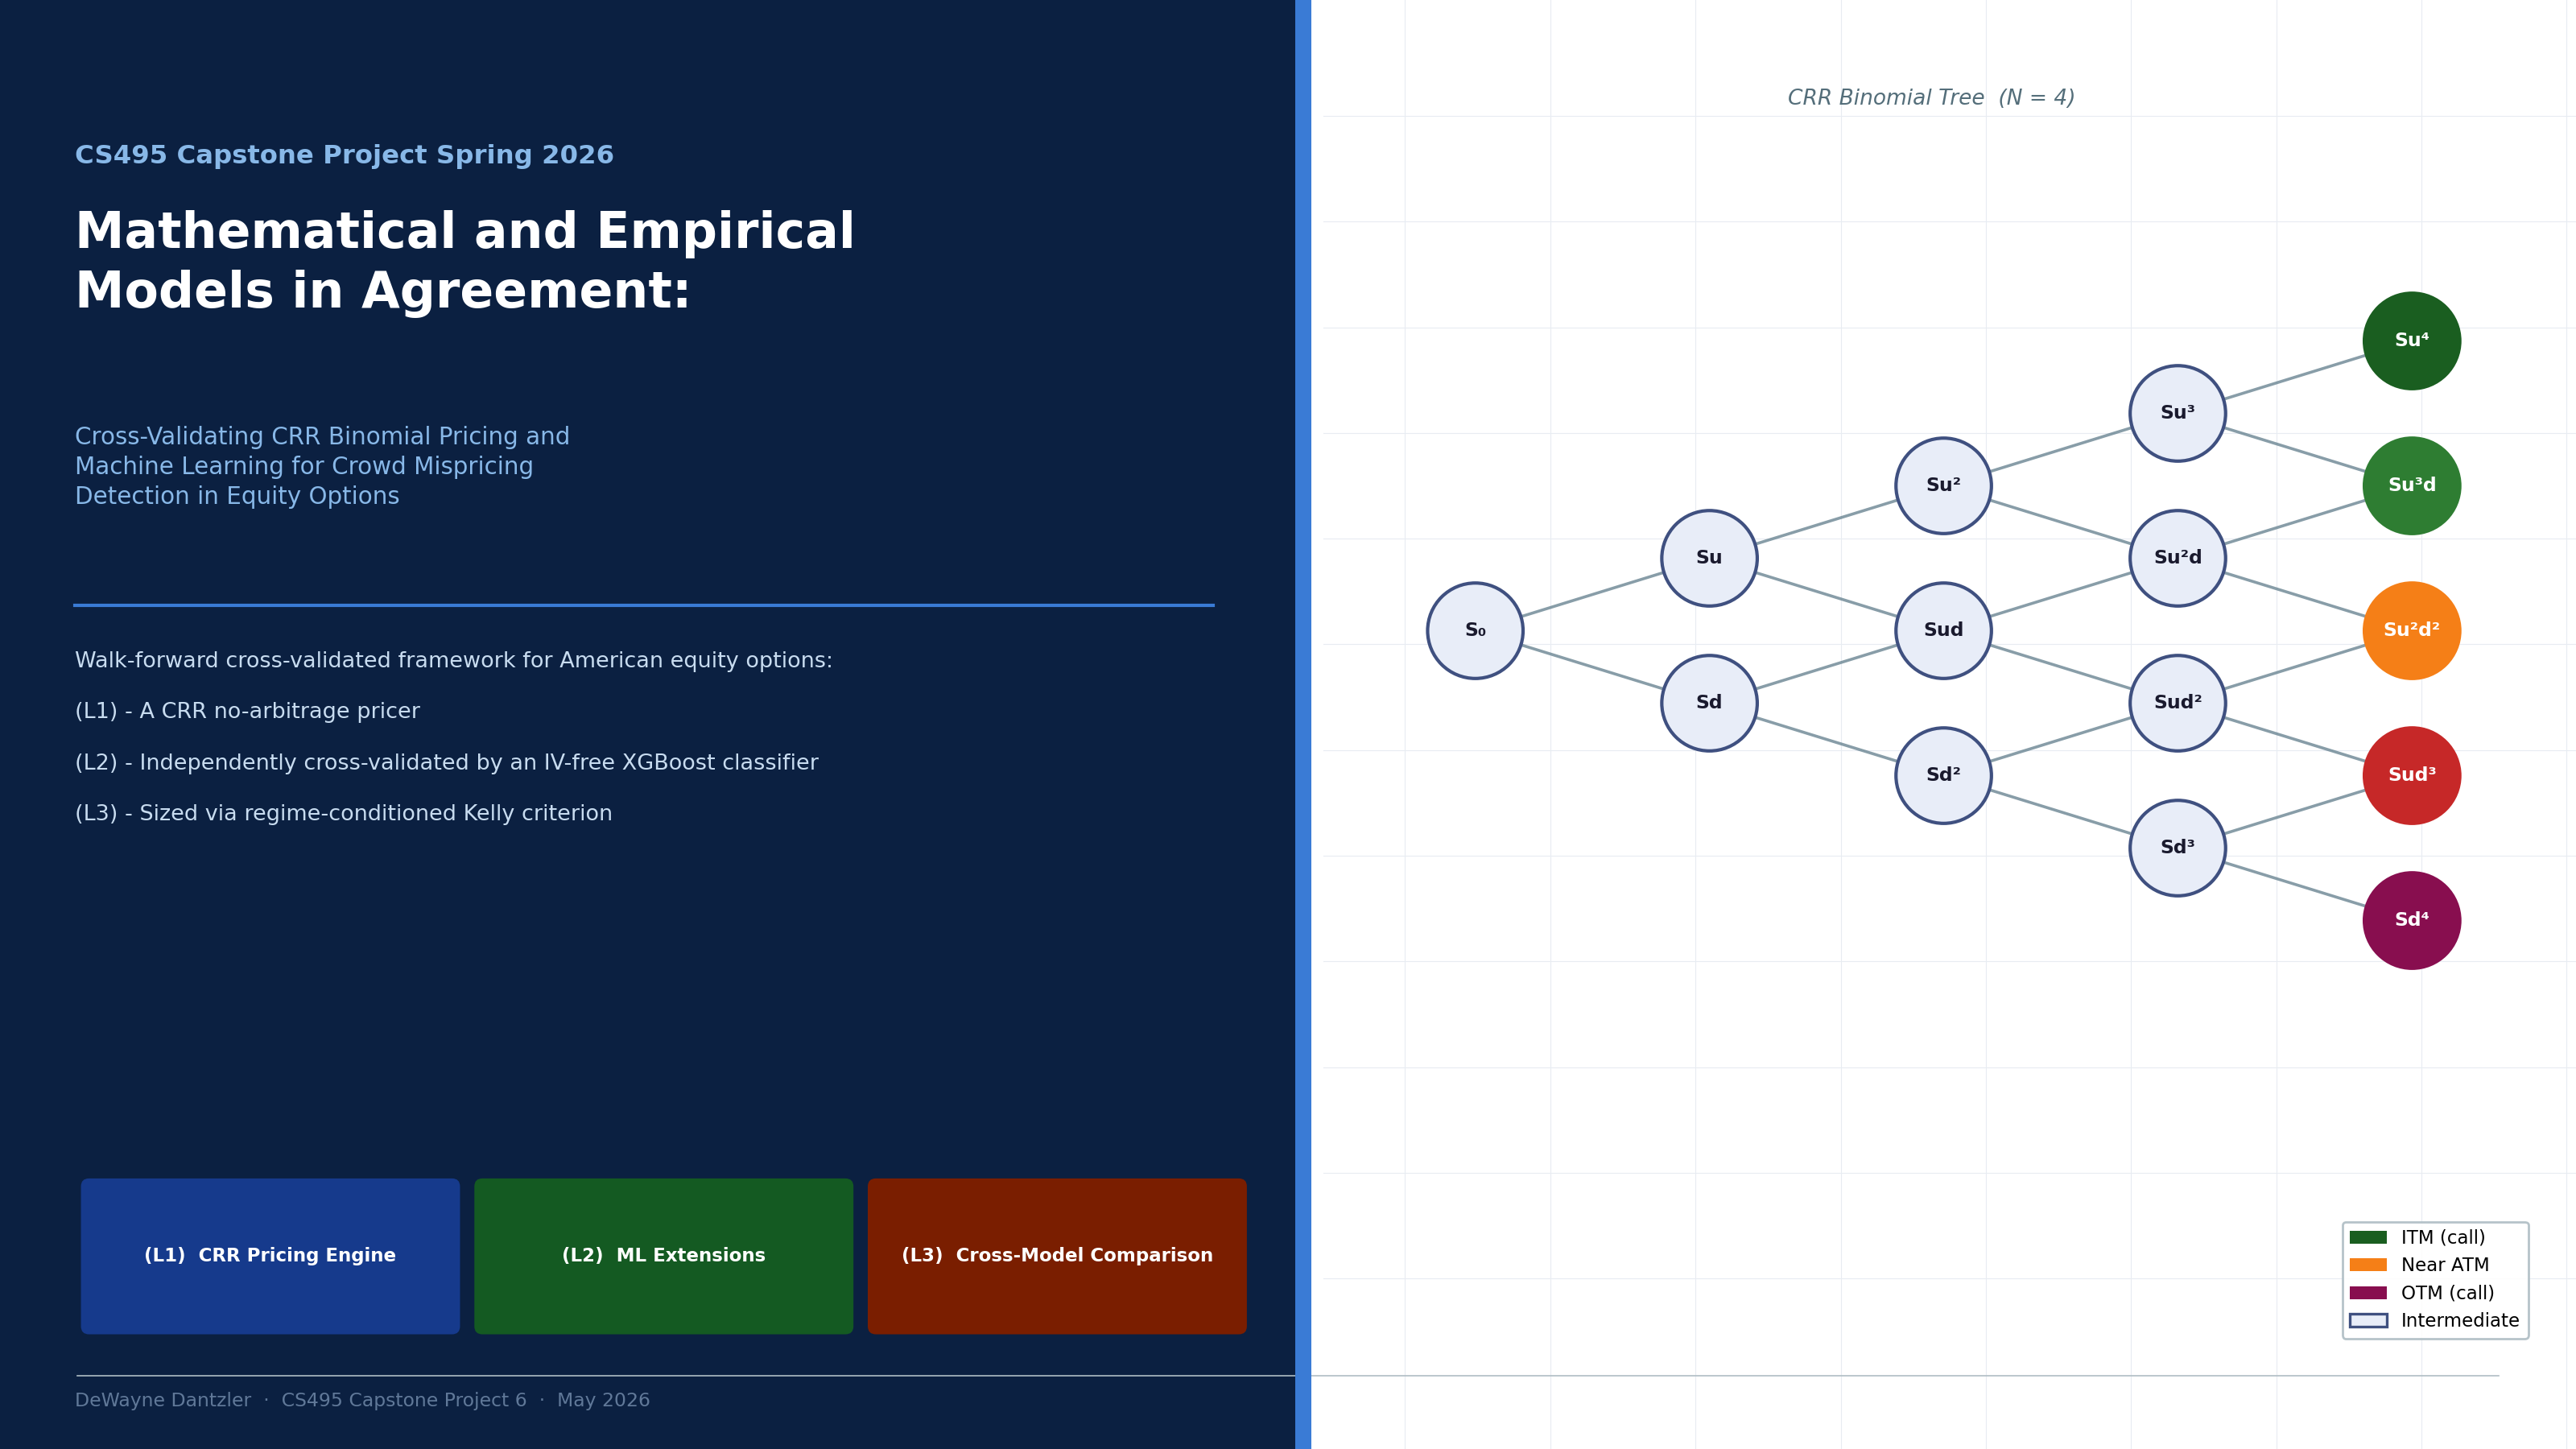
\includegraphics[width=20cm, keepaspectratio]{previews/cover_slide.png}};
\end{tikzpicture}

\vspace*{14cm}

% ══════════════════════════════════════════════════════════════════════════════
%  BODY — two-column layout (main + summary sidebar)
% ══════════════════════════════════════════════════════════════════════════════
\begin{columns}[T]

% ──────────────────────────────────────────────────────────────────────────────
%  MAIN CONTENT COLUMN (left, ~65 %)
% ──────────────────────────────────────────────────────────────────────────────
\column{0.65\linewidth}

% ── Row 1 — Forward Pass + Backward Induction (slides 6 and 7 figures) ───────
\begin{block}{Methodology in Action: Contract A Forward + Backward}
  \begin{columns}[T]
    \column{0.49\linewidth}
      \centering
      \textbf{\large Forward Pass}\\[0.15cm]
      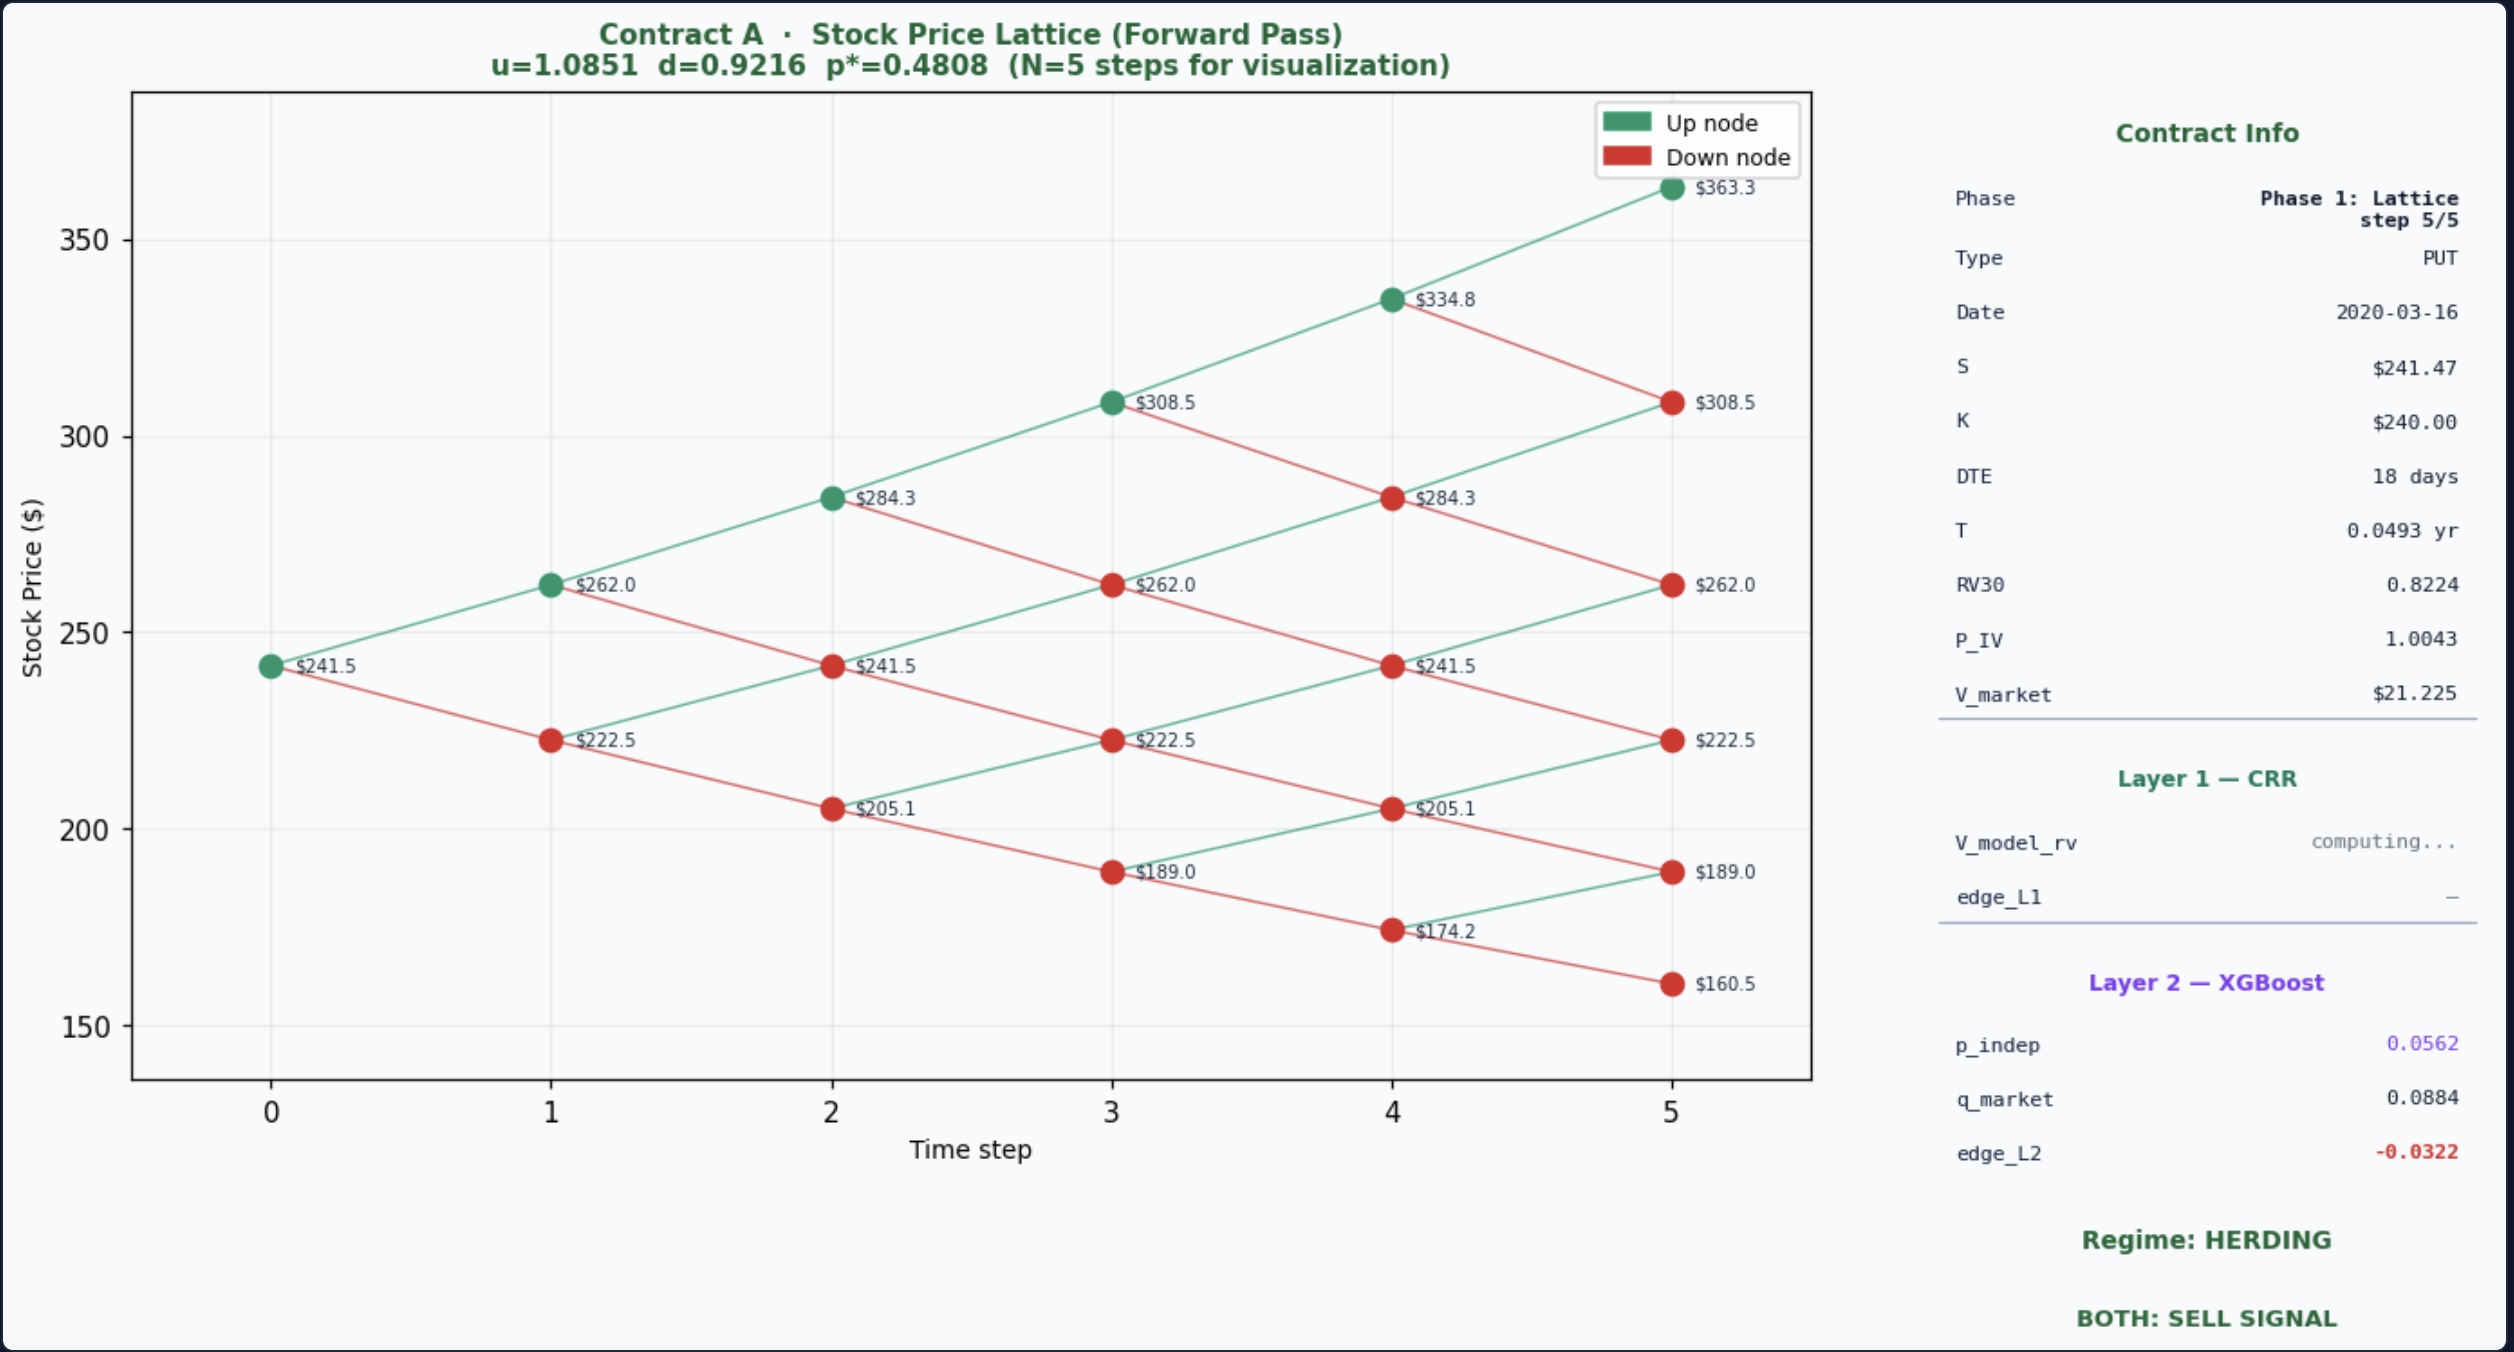
\includegraphics[width=\linewidth,keepaspectratio]
        {previews/Slide-Forward-Pass.png}\\[0.15cm]
      {\footnotesize Stock-price lattice using
       $u = e^{\sigma\sqrt{\Delta t}}$, $d = 1/u$, $p^{*} = 0.481$}
    \column{0.49\linewidth}
      \centering
      \textbf{\large Backward Induction}\\[0.15cm]
      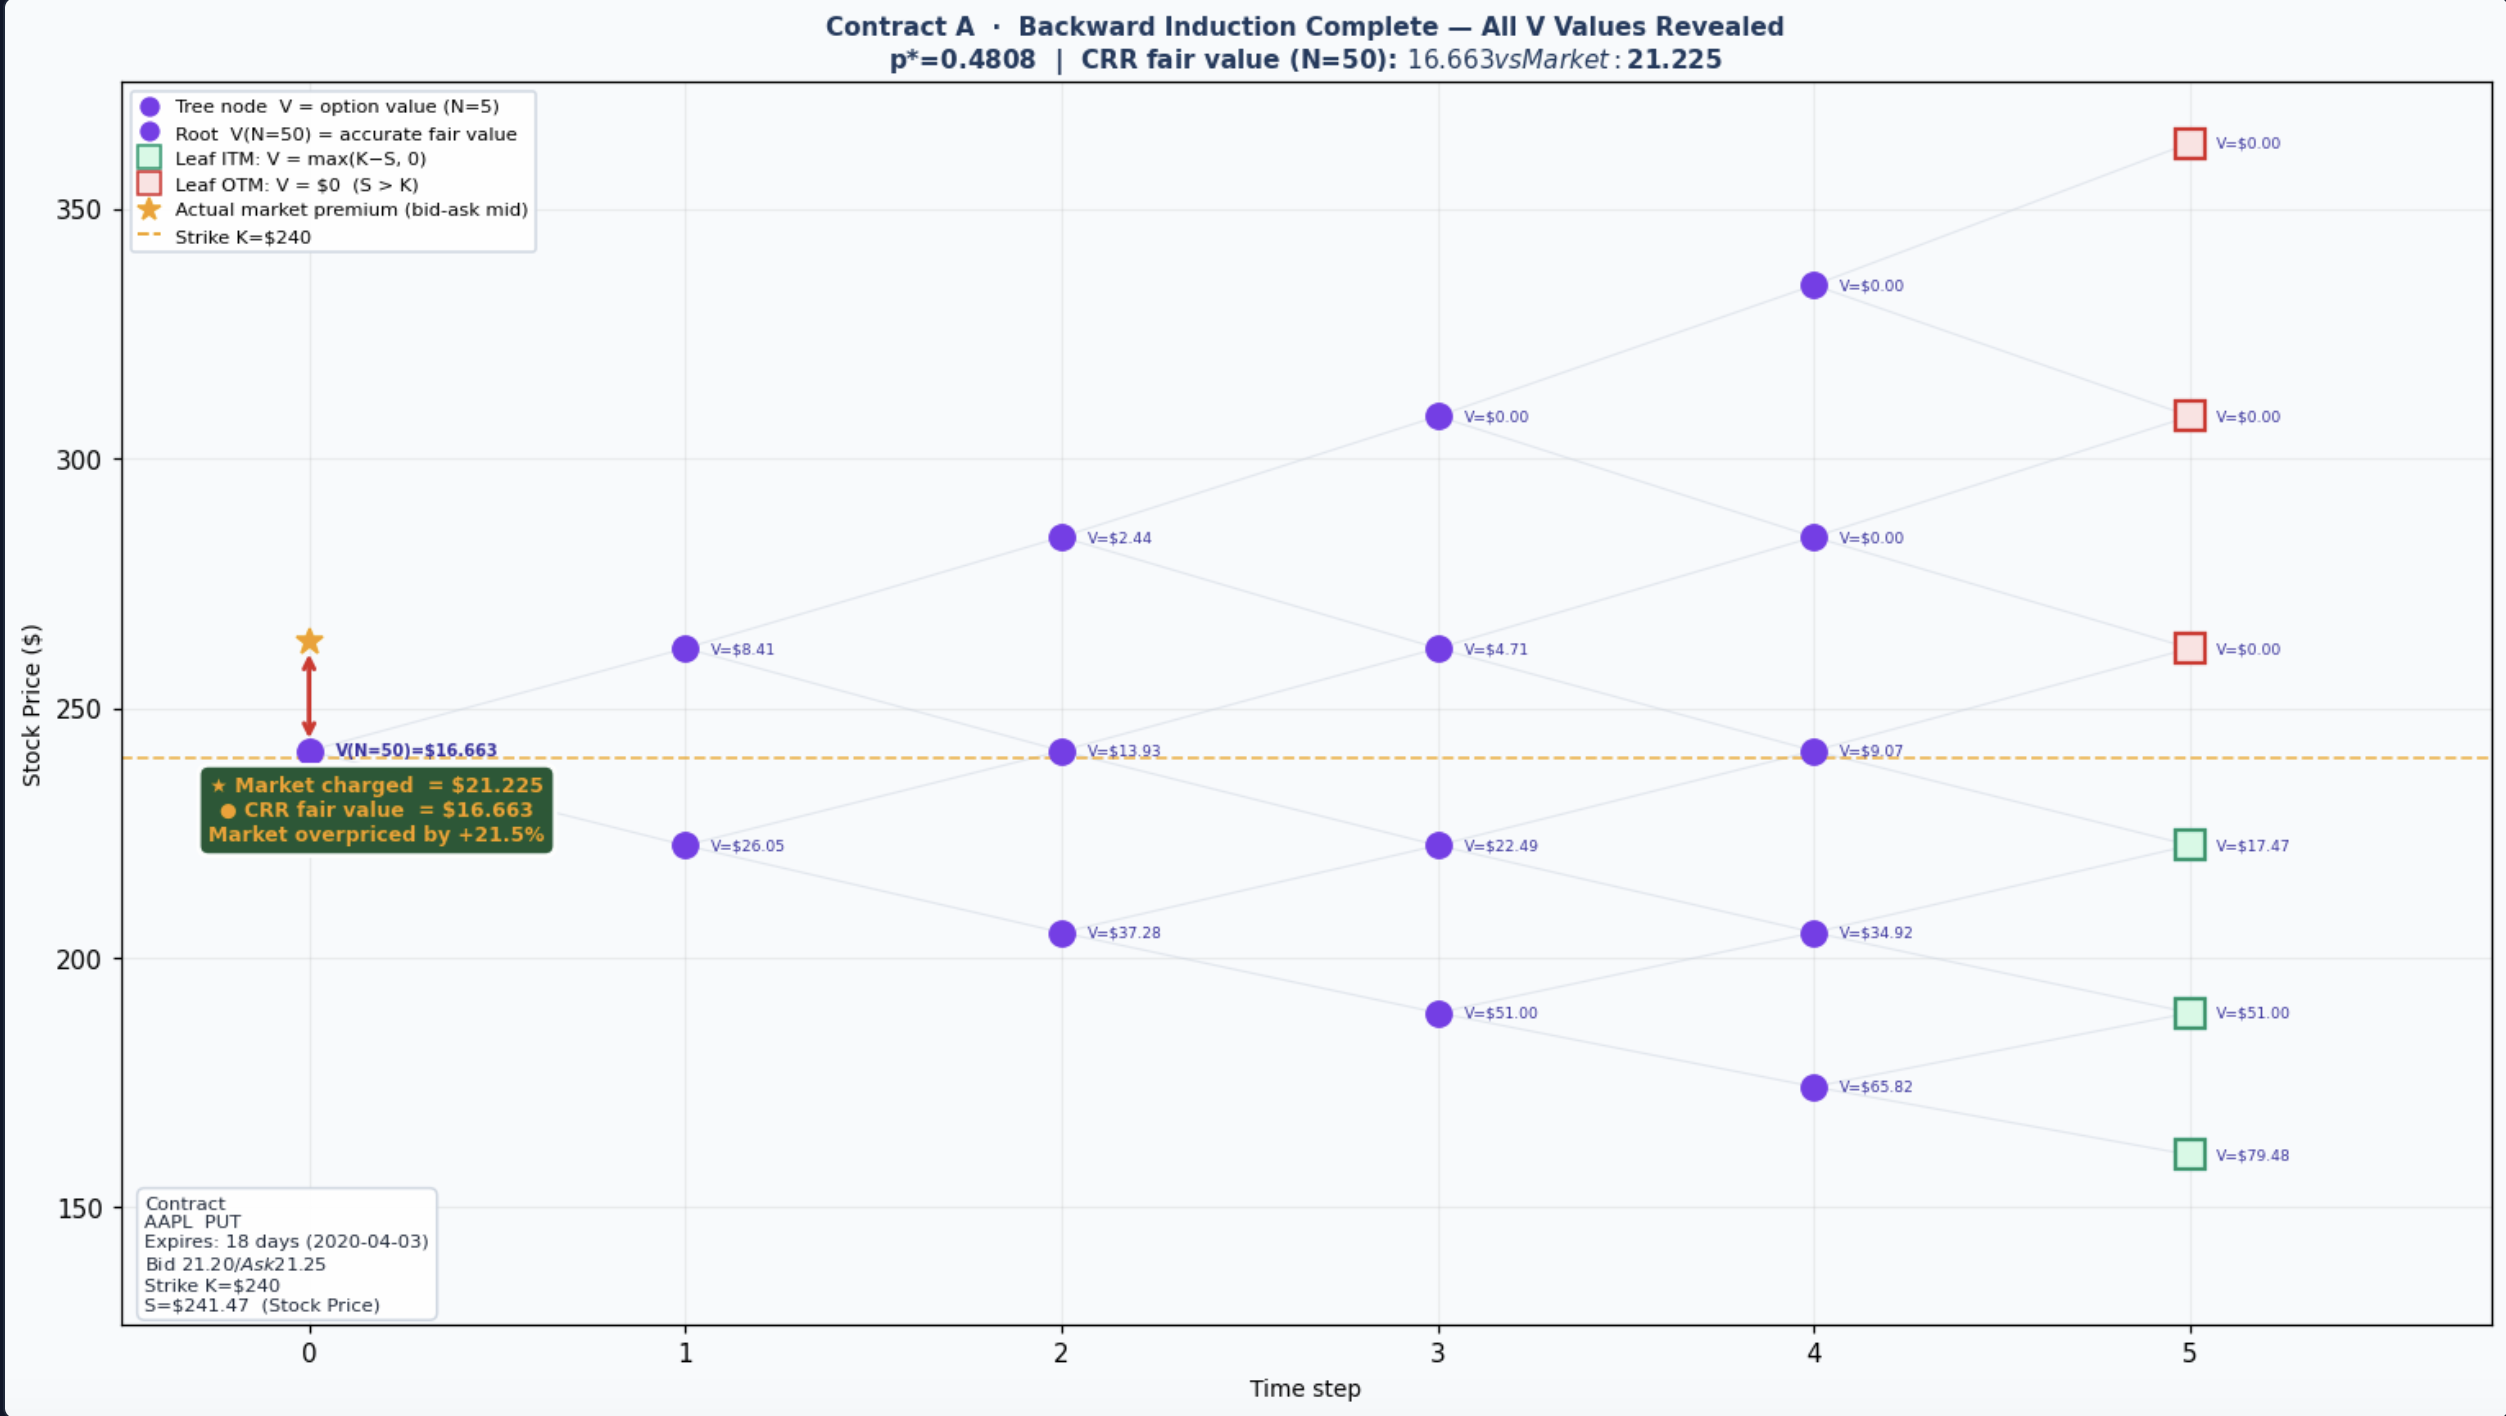
\includegraphics[width=\linewidth,keepaspectratio]
        {previews/Slide-Backward-Pass.png}\\[0.15cm]
      {\footnotesize At every node:
       $V = \max\bigl(\text{intrinsic},\ e^{-r\Delta t}(p^{*}V_{u} + qV_{d})\bigr)$}
  \end{columns}
\end{block}

% ── Row 2 — Contract A Result (slide 8 figure) ───────────────────────────────
\begin{block}{Contract A Result: Two Independent Models Agree}
  \centering
  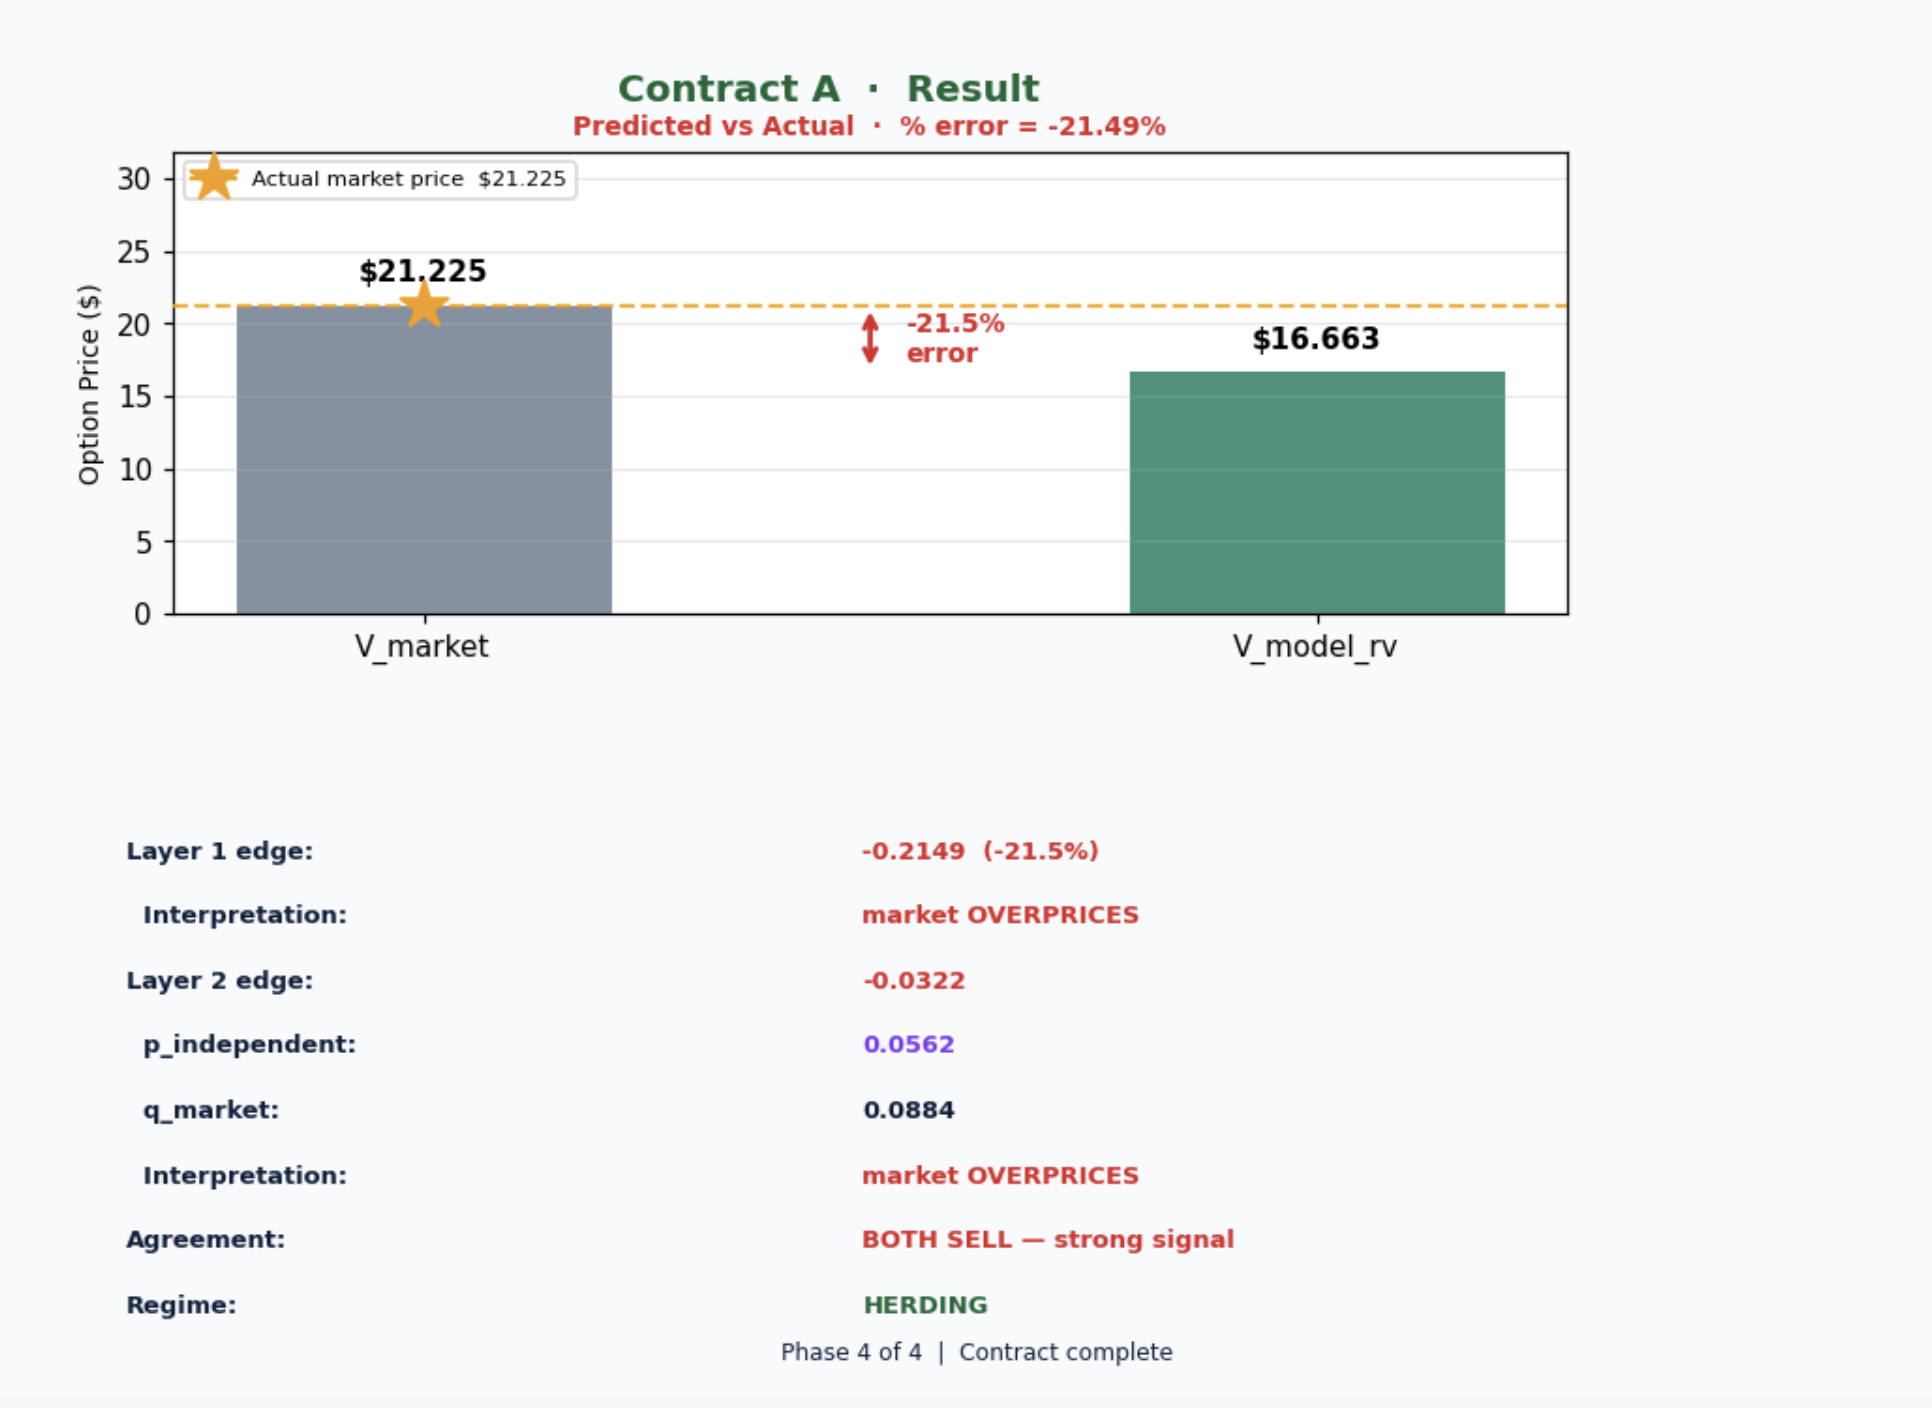
\includegraphics[height=14cm,keepaspectratio]
    {previews/Slide-Option-Pricing-Results.png}\\[0.2cm]
  {\small
   Layer 1 (CRR) edge $= -21.5\%$ and Layer 2 (XGBoost) edge $= -3.2\%$:
   \textbf{both models say SELL} on this real AAPL put.\ \
   Same conclusion reached by completely independent methods.}
\end{block}

% ── Row 3 — Cross-Model Edge Agreement (hero scatter) ────────────────────────
\begin{block}{Cross-Model Edge Agreement on AAPL Options}
  \centering
  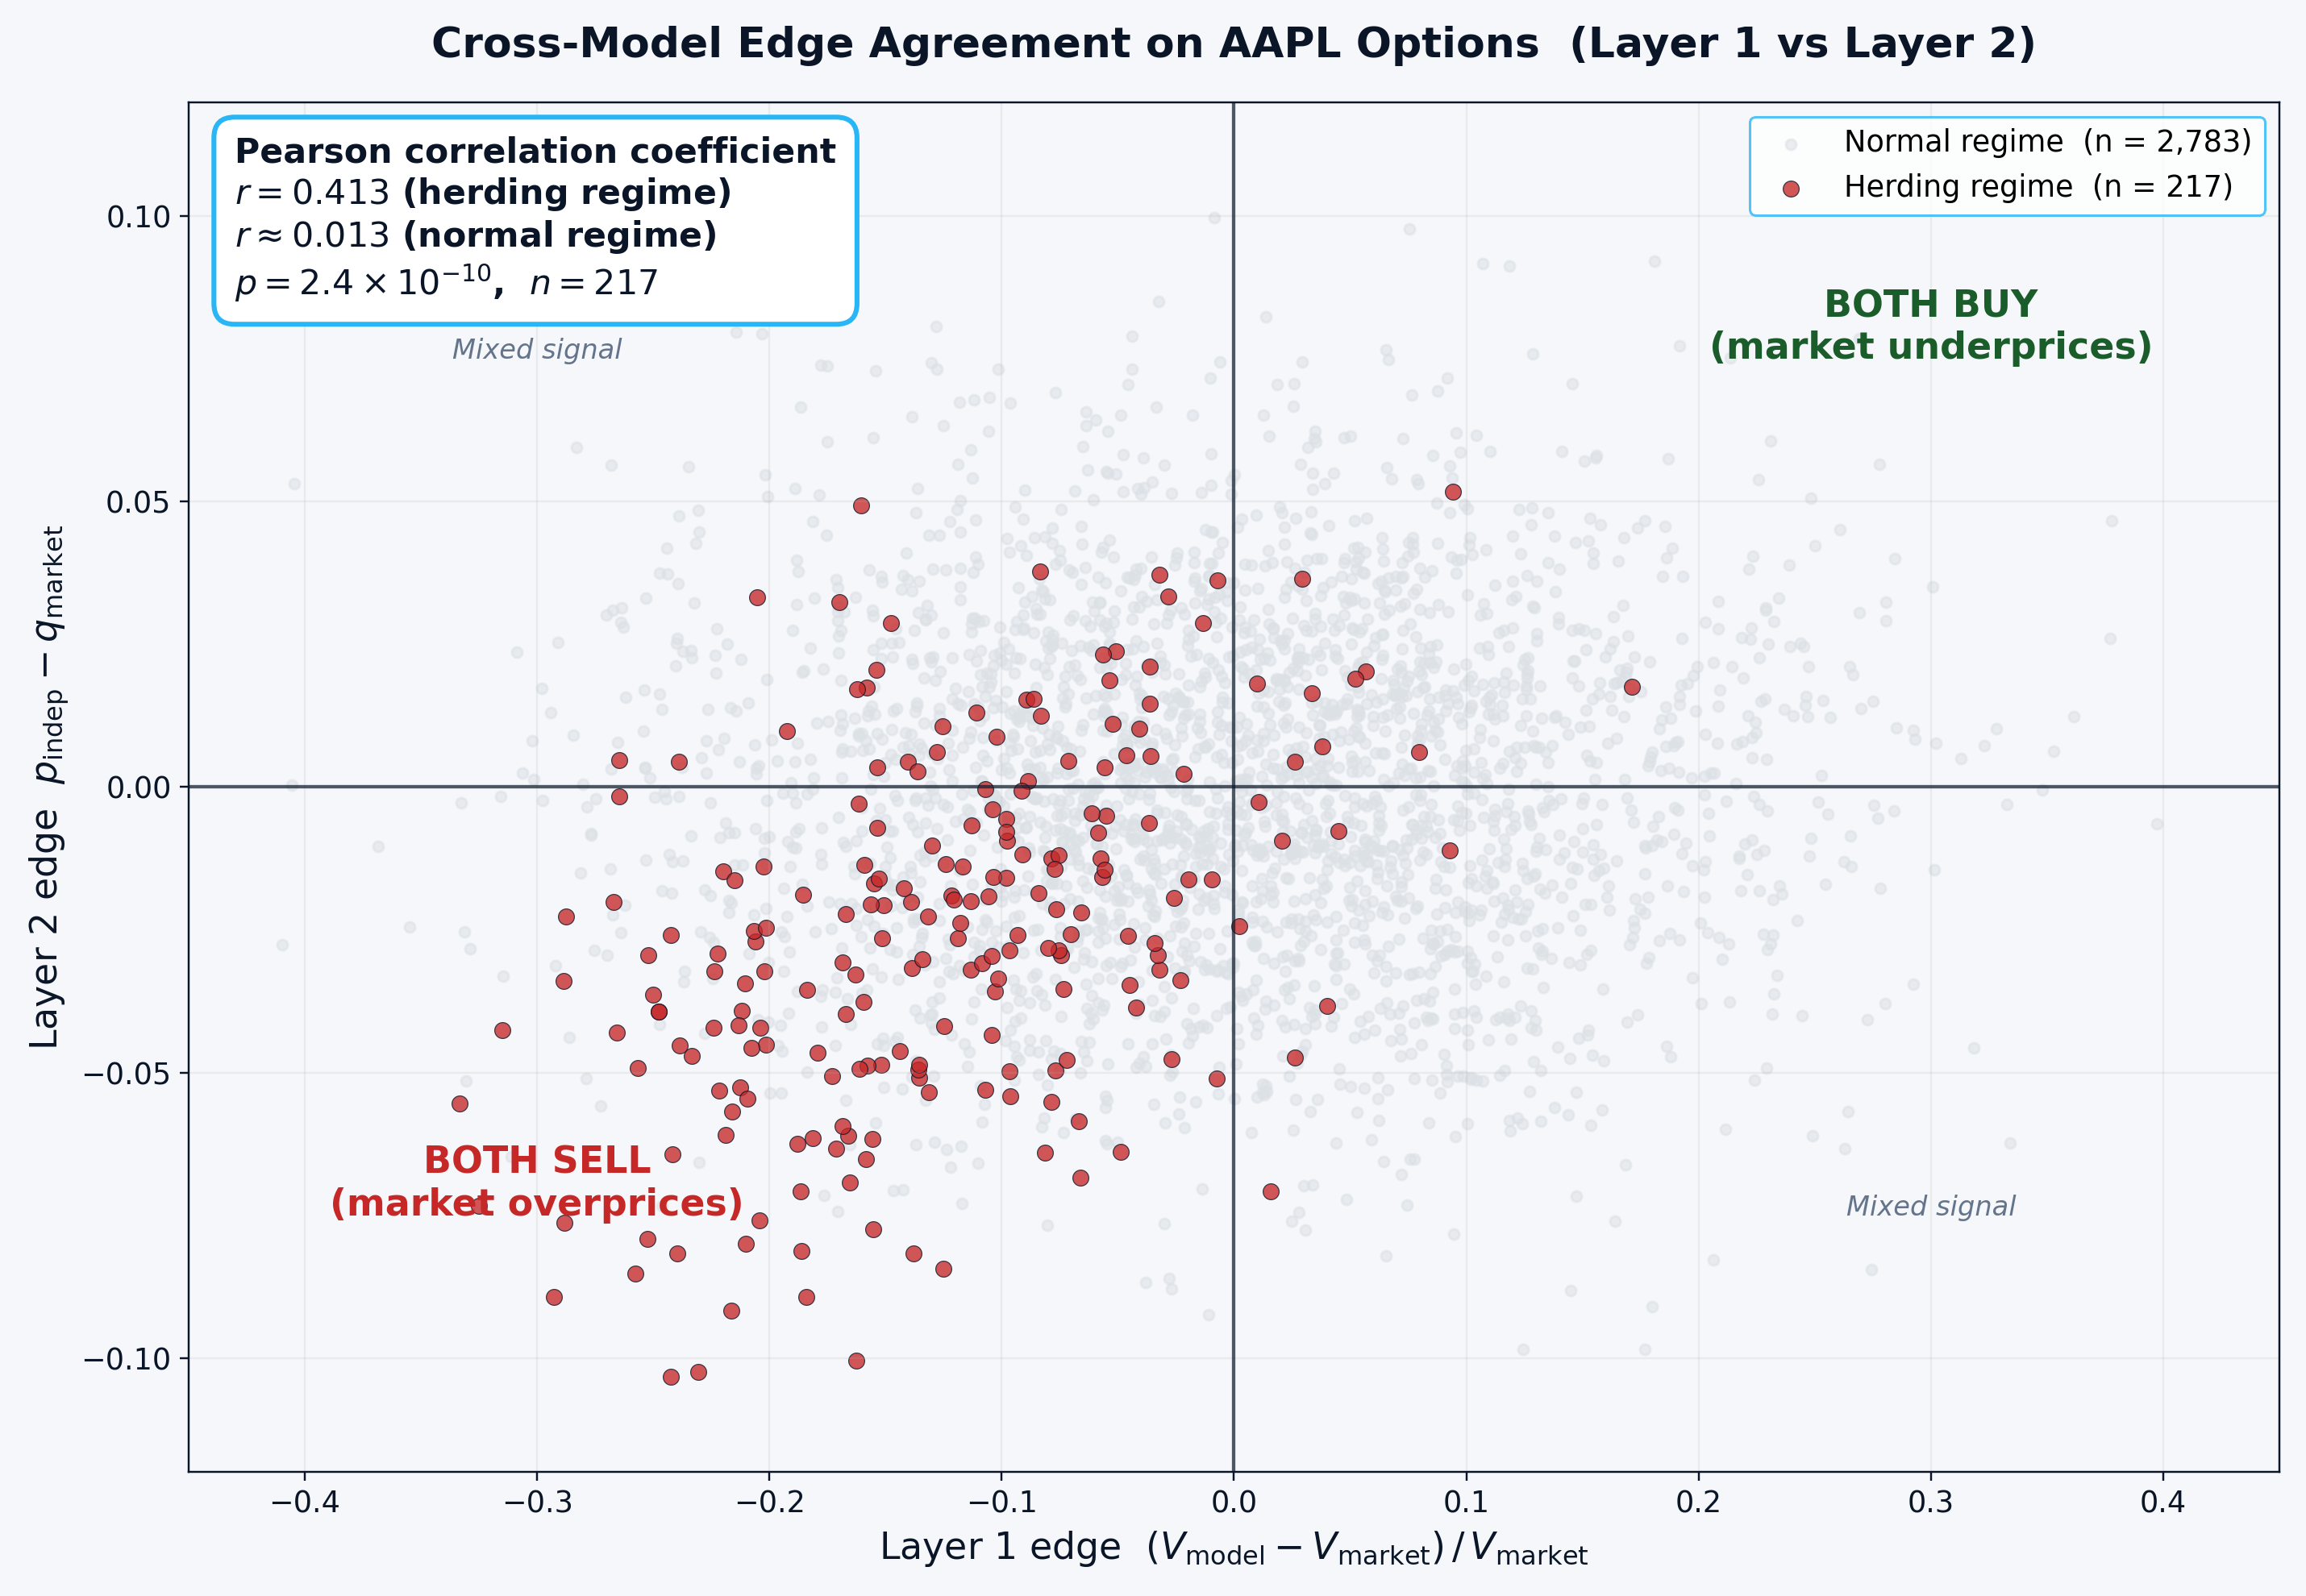
\includegraphics[height=14cm,keepaspectratio]
    {previews/poster/poster_hero_scatter.png}\\[0.2cm]
  {\small
   Pearson correlation coefficient
   $r = 0.413$ (herding) vs $r \approx 0$ (normal),
   $p = 2.4\times10^{-10}$.\ \
   Agreement concentrated in the herding regime --- the empirical
   fingerprint of Samuelson macro-inefficiency.}
\end{block}

% ── Row 4 — Methodology (slide 4 PDF page embed) ─────────────────────────────
\begin{block}{Contribution \& Methodology (Slide 4)}
  \centering
  \includegraphics[page=4, width=\linewidth, keepaspectratio]
    {CS495_Capstone_Presentation.pdf}
\end{block}

% ── Row 5 — Live Demo (calculator screenshot from slide 12) ──────────────────
\begin{block}{Live Demo: Interactive CRR Binomial Pricing Calculator}
  \centering
  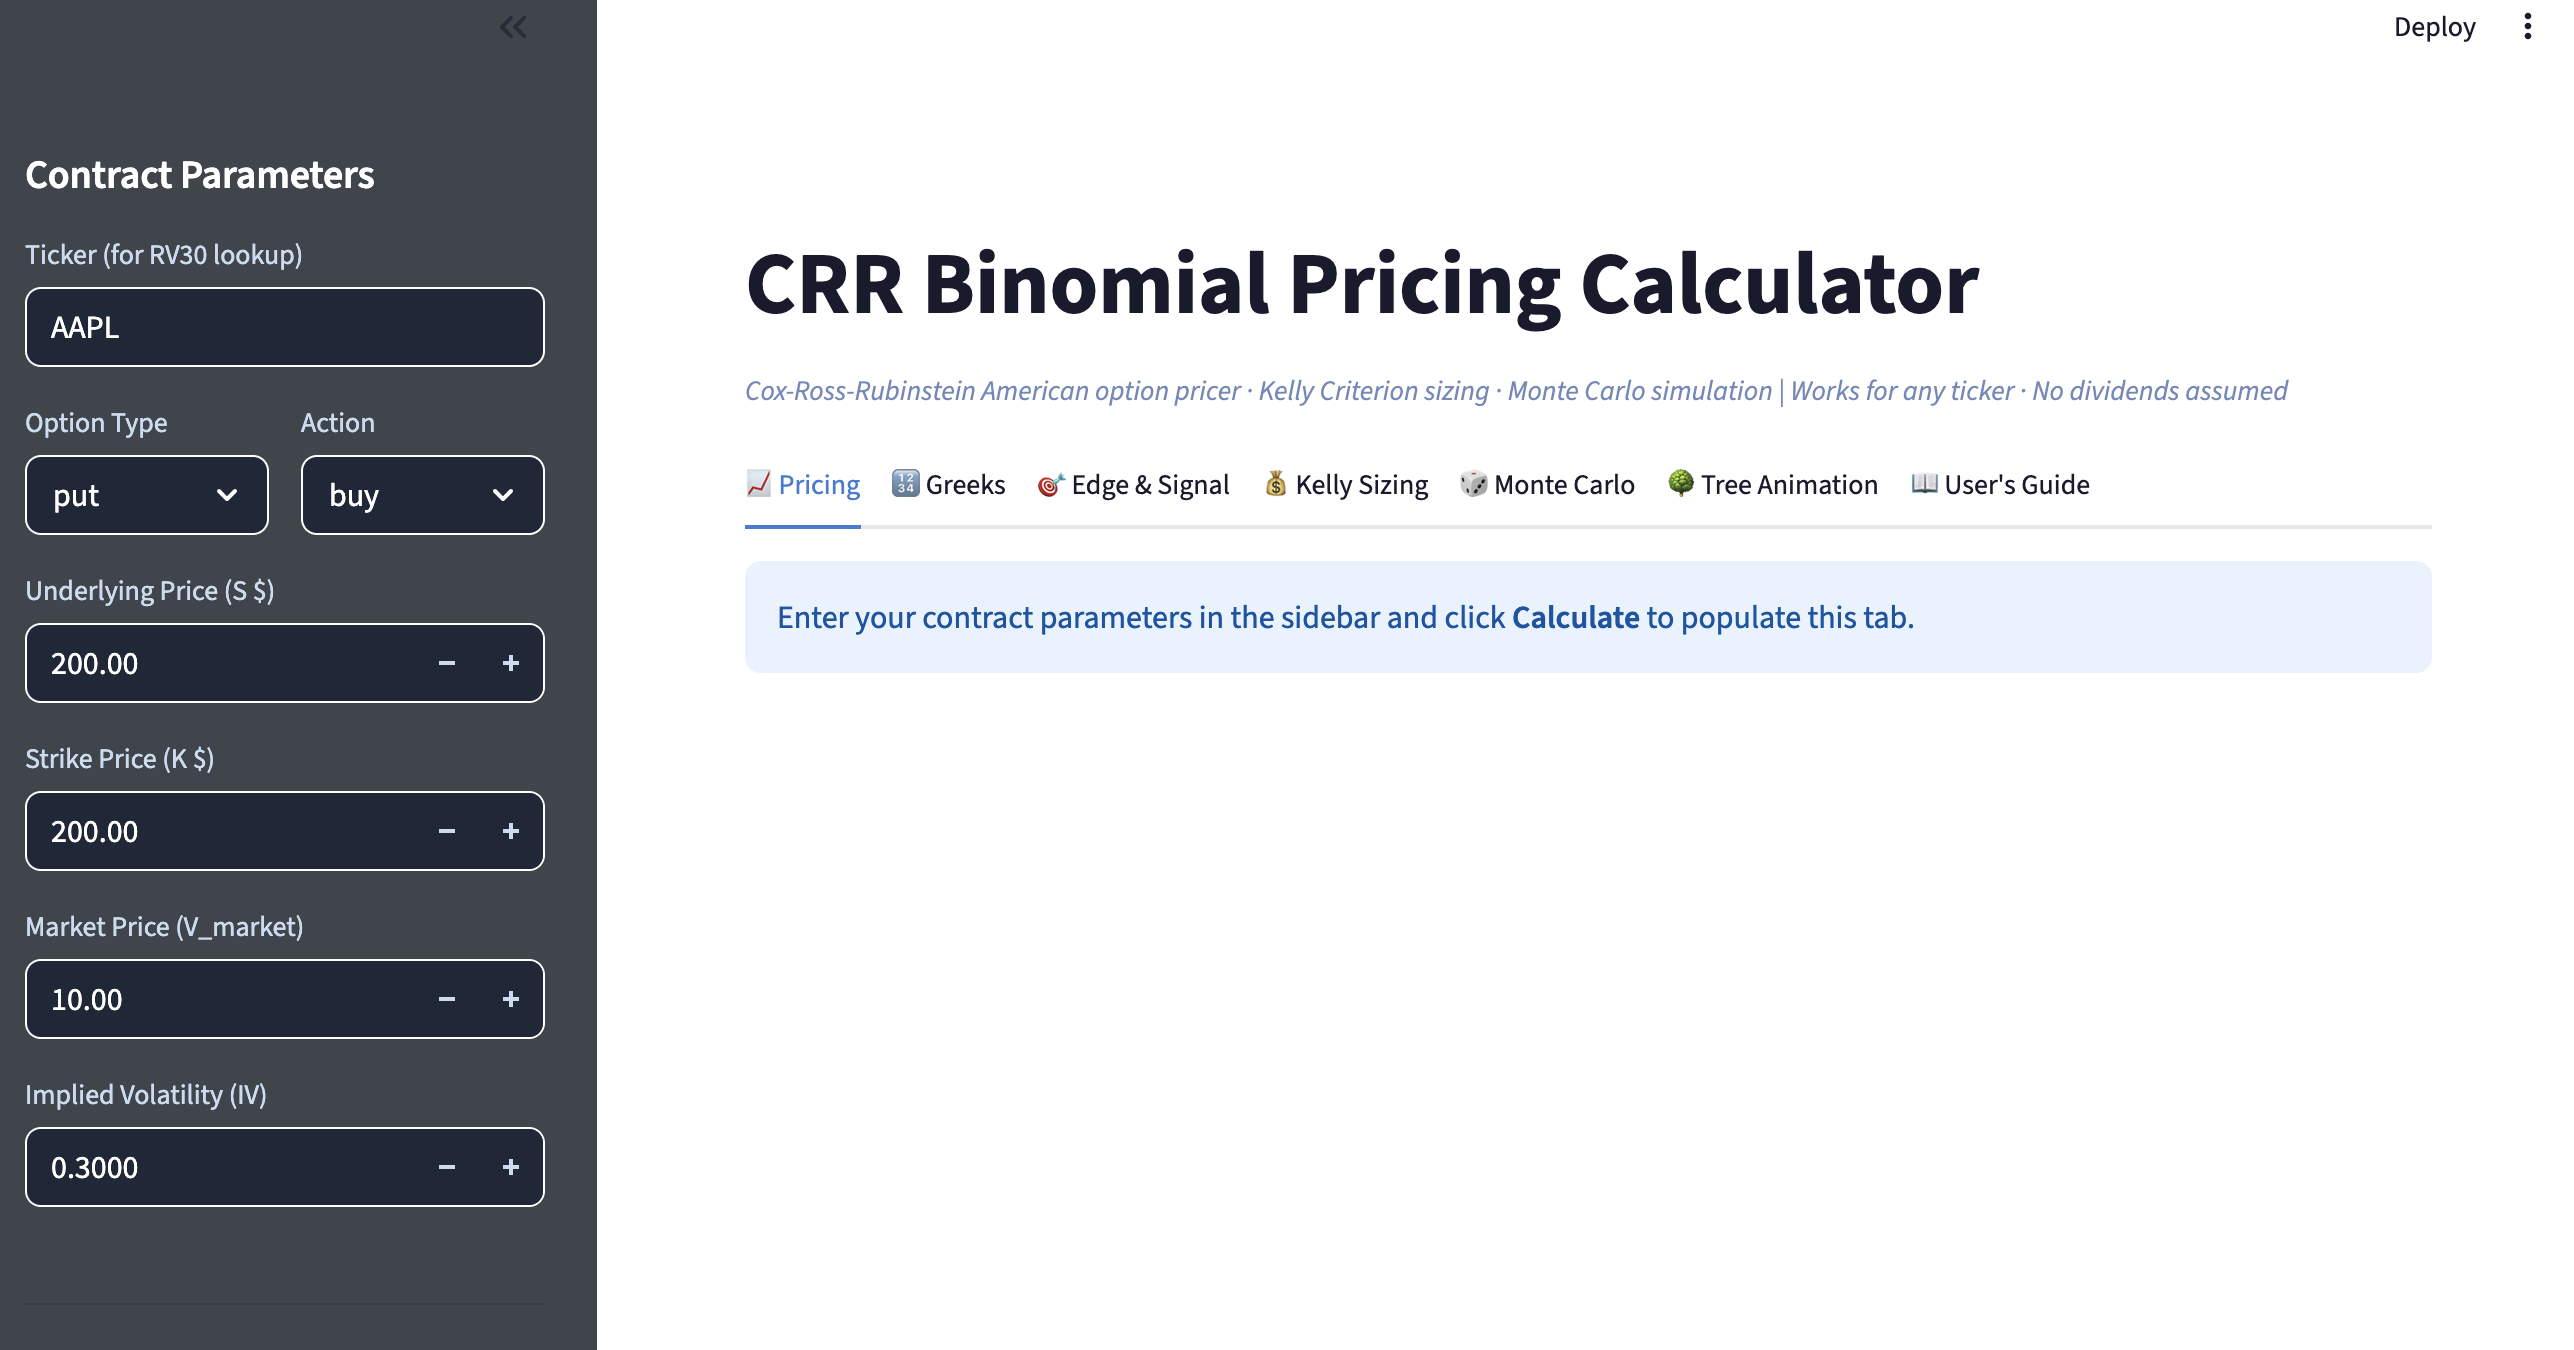
\includegraphics[width=\linewidth,keepaspectratio]
    {previews/crr-binomial-pricing-calculator.png}\\[0.15cm]
  {\small
   Streamlit application $\cdot$ runs locally on any laptop with Python 3.13
   $\cdot$ ticker-agnostic (live RV30 fetch via yfinance) $\cdot$
   embedded user's guide PDF.}
\end{block}

% ──────────────────────────────────────────────────────────────────────────────
%  SIDEBAR COLUMN (right, ~33 %) — full-height Project Summary
% ──────────────────────────────────────────────────────────────────────────────
\column{0.33\linewidth}

\begin{block}{Project Summary}
  \footnotesize

  \textbf{\color{navymid} The question.}\ \
  When an options pricing model produces a theoretical fair value that
  diverges from the observed market premium, is that divergence large
  enough --- and reliable enough --- to justify a trade? If so, how
  much of the available capital should be committed, given the
  inherent uncertainty of the model?

  \vspace{0.4cm}
  \textbf{\color{navymid} Why it matters.}\ \
  Options markets aggregate beliefs into prices the same way prediction
  markets do, but behavioral forces (herding, vol-risk premium,
  out-of-the-money skew) distort those prices in predictable ways.
  The gap between a model's fair value and the observed premium is
  potentially exploitable by a disciplined, model-driven strategy.

  \vspace{0.4cm}
  \textbf{\color{navymid} Approach.}\ \
  A Python implementation of the Cox--Ross--Rubinstein (CRR)
  \emph{American} binomial option pricer is built and validated
  against live AMD option chain data captured from Fidelity in
  April 2026. The pricer's output is treated as an independent
  probability estimate and combined with Kelly Criterion sizing
  for disciplined risk-controlled trade allocation.

  \vspace{0.4cm}
  \textbf{\color{navymid} Cross-validation.}\ \
  Two completely independent models are deployed in parallel:
  \begin{itemize}
    \setlength{\itemsep}{0.18cm}
    \item \textbf{Layer 1 (CRR no-arbitrage math)} --- theoretical fair
          value derived from realized volatility ($\sigma = $ RV30).
    \item \textbf{Layer 2 (XGBoost ML classifier)} --- empirical
          ITM/OTM probability estimate, trained on 101{,}535 historical
          AAPL contracts.
  \end{itemize}
  Their \emph{agreement} on which contracts the market misprices
  constitutes mutual validation: neither layer is trained on the
  other, so concurrent signals come from shared underlying reality.

  \vspace{0.4cm}
  \textbf{\color{navymid} Key result.}\ \
  Across 3{,}000 sampled AAPL contracts, the two layers' edge signals
  agree strongly in the \textbf{herding regime} (Pearson
  $r = 0.413$, $p = 2.4\times10^{-10}$) and not at all in the
  \textbf{normal regime} ($r \approx 0$). Agreement is concentrated
  precisely where behavioral-finance theory predicts crowd bias is
  strongest --- the empirical fingerprint of Samuelson's
  macro-inefficiency thesis.

  \vspace{0.4cm}
  \textbf{\color{navymid} Datasets.}\ \
  AMD live chain (April 2026, 4 trade tickets at $\sigma \approx 64\%$)
  $\cdot$ AAPL 2016--2020 Kaggle (101{,}535 contracts).

  \vspace{0.4cm}
  \textbf{\color{navymid} Tech stack.}\ \
  Python 3.13 $\cdot$ NumPy $\cdot$ pandas $\cdot$ XGBoost $\cdot$
  scikit-learn $\cdot$ matplotlib $\cdot$ Streamlit $\cdot$ yfinance
  $\cdot$ Poetry $\cdot$ LaTeX/Beamer $\cdot$ Git\,/\,GitHub.

  \vspace{0.4cm}
  \textbf{\color{navymid} Conclusions.}
  \begin{itemize}
    \setlength{\itemsep}{0.18cm}
    \item Mathematics and ML, working independently, reach the
          \emph{same} mispricing conclusion in the regime theory
          predicts.
    \item The framework is a falsifiable test of EMH
          (Fama 1970): in a Fama-efficient market, this agreement
          could not persist.
    \item Kelly sizing converts the detected edge into capital
          allocation with controlled drawdown.
    \item Fully reproducible: one \texttt{make run-all} command
          regenerates every artifact end-to-end.
  \end{itemize}
\end{block}

\end{columns}

% ══════════════════════════════════════════════════════════════════════════════
%  FOOTER BAND — references + QR
% ══════════════════════════════════════════════════════════════════════════════
\begin{tikzpicture}[remember picture, overlay]
  \fill[navydark] ($(current page.south west) + (0, 4.5cm)$)
                  rectangle (current page.south east);

  \fill[goldaccent] (current page.south west)
                    rectangle ($(current page.south west) + (0.8cm, 4.5cm)$);

  \node[anchor=north west, text=skybluelight,
        font=\sffamily\fontsize{14}{20}, text width=68cm]
    at ($(current page.south west) + (2.5cm, 4.0cm)$)
    {\textbf{Key references:}\ \
     Black \& Scholes (1973) $\cdot$
     Cox--Ross--Rubinstein (1979) $\cdot$
     Fama (1970) $\cdot$
     Carr \& Wu (2009) $\cdot$
     Kelly (1956) $\cdot$
     MacLean--Thorp--Ziemba (2010)\\[0.2cm]
     \textbf{Contact:}\
     \texttt{dewayne.dantzler@bellevuecollege.edu}\\[0.2cm]
     \textbf{Full report and code repository:}\
     \texttt{github.com/dantzlerdc/CS495-Deep-Scholar}};

  \node[anchor=south east, fill=white, inner sep=0.3cm,
        rounded corners=4pt]
    at ($(current page.south east) + (-2.5cm, 0.6cm)$)
    {\qrcode[height=3.2cm]{https://github.com/dantzlerdc/CS495-Deep-Scholar}};

  \node[anchor=south, text=skybluelight,
        font=\sffamily\fontsize{12}{14}\bfseries]
    at ($(current page.south east) + (-5.3cm, 0.2cm)$)
    {Scan for repo};
\end{tikzpicture}

\end{frame}

\end{document}
